\documentclass[../Results.tex]{subfiles}

\begin{document}
	In this section we present the maps for the flux-weighted velocity centroid and the flux-weighted velocity dispersion of all of the extended emission line to get an indication of the centroid velocity and width of the emission line for each spatial location. Different emission line traces different gas component. We use ly$\alpha$ to trace cool gas($10^{4}$K) and use CIV($\lambda1549$),HeII($\lambda1640$) emission to trace warm gas($10^{5}$K).  These resolved kinematic maps give us the opportunity to detect kinematic patterns, e.g. evidence for rotation, inflows or outflows and help us to have a deep insight look to the physics of this nebula. We filter the spectra with lowpass filter to reduce the noise, this procedure can help us to construct a more clear velocity and velocity dispersion map, we show the results in Fig. \ref{kinematicsmap}
	 \begin{figure*}[htp]
		\centering
		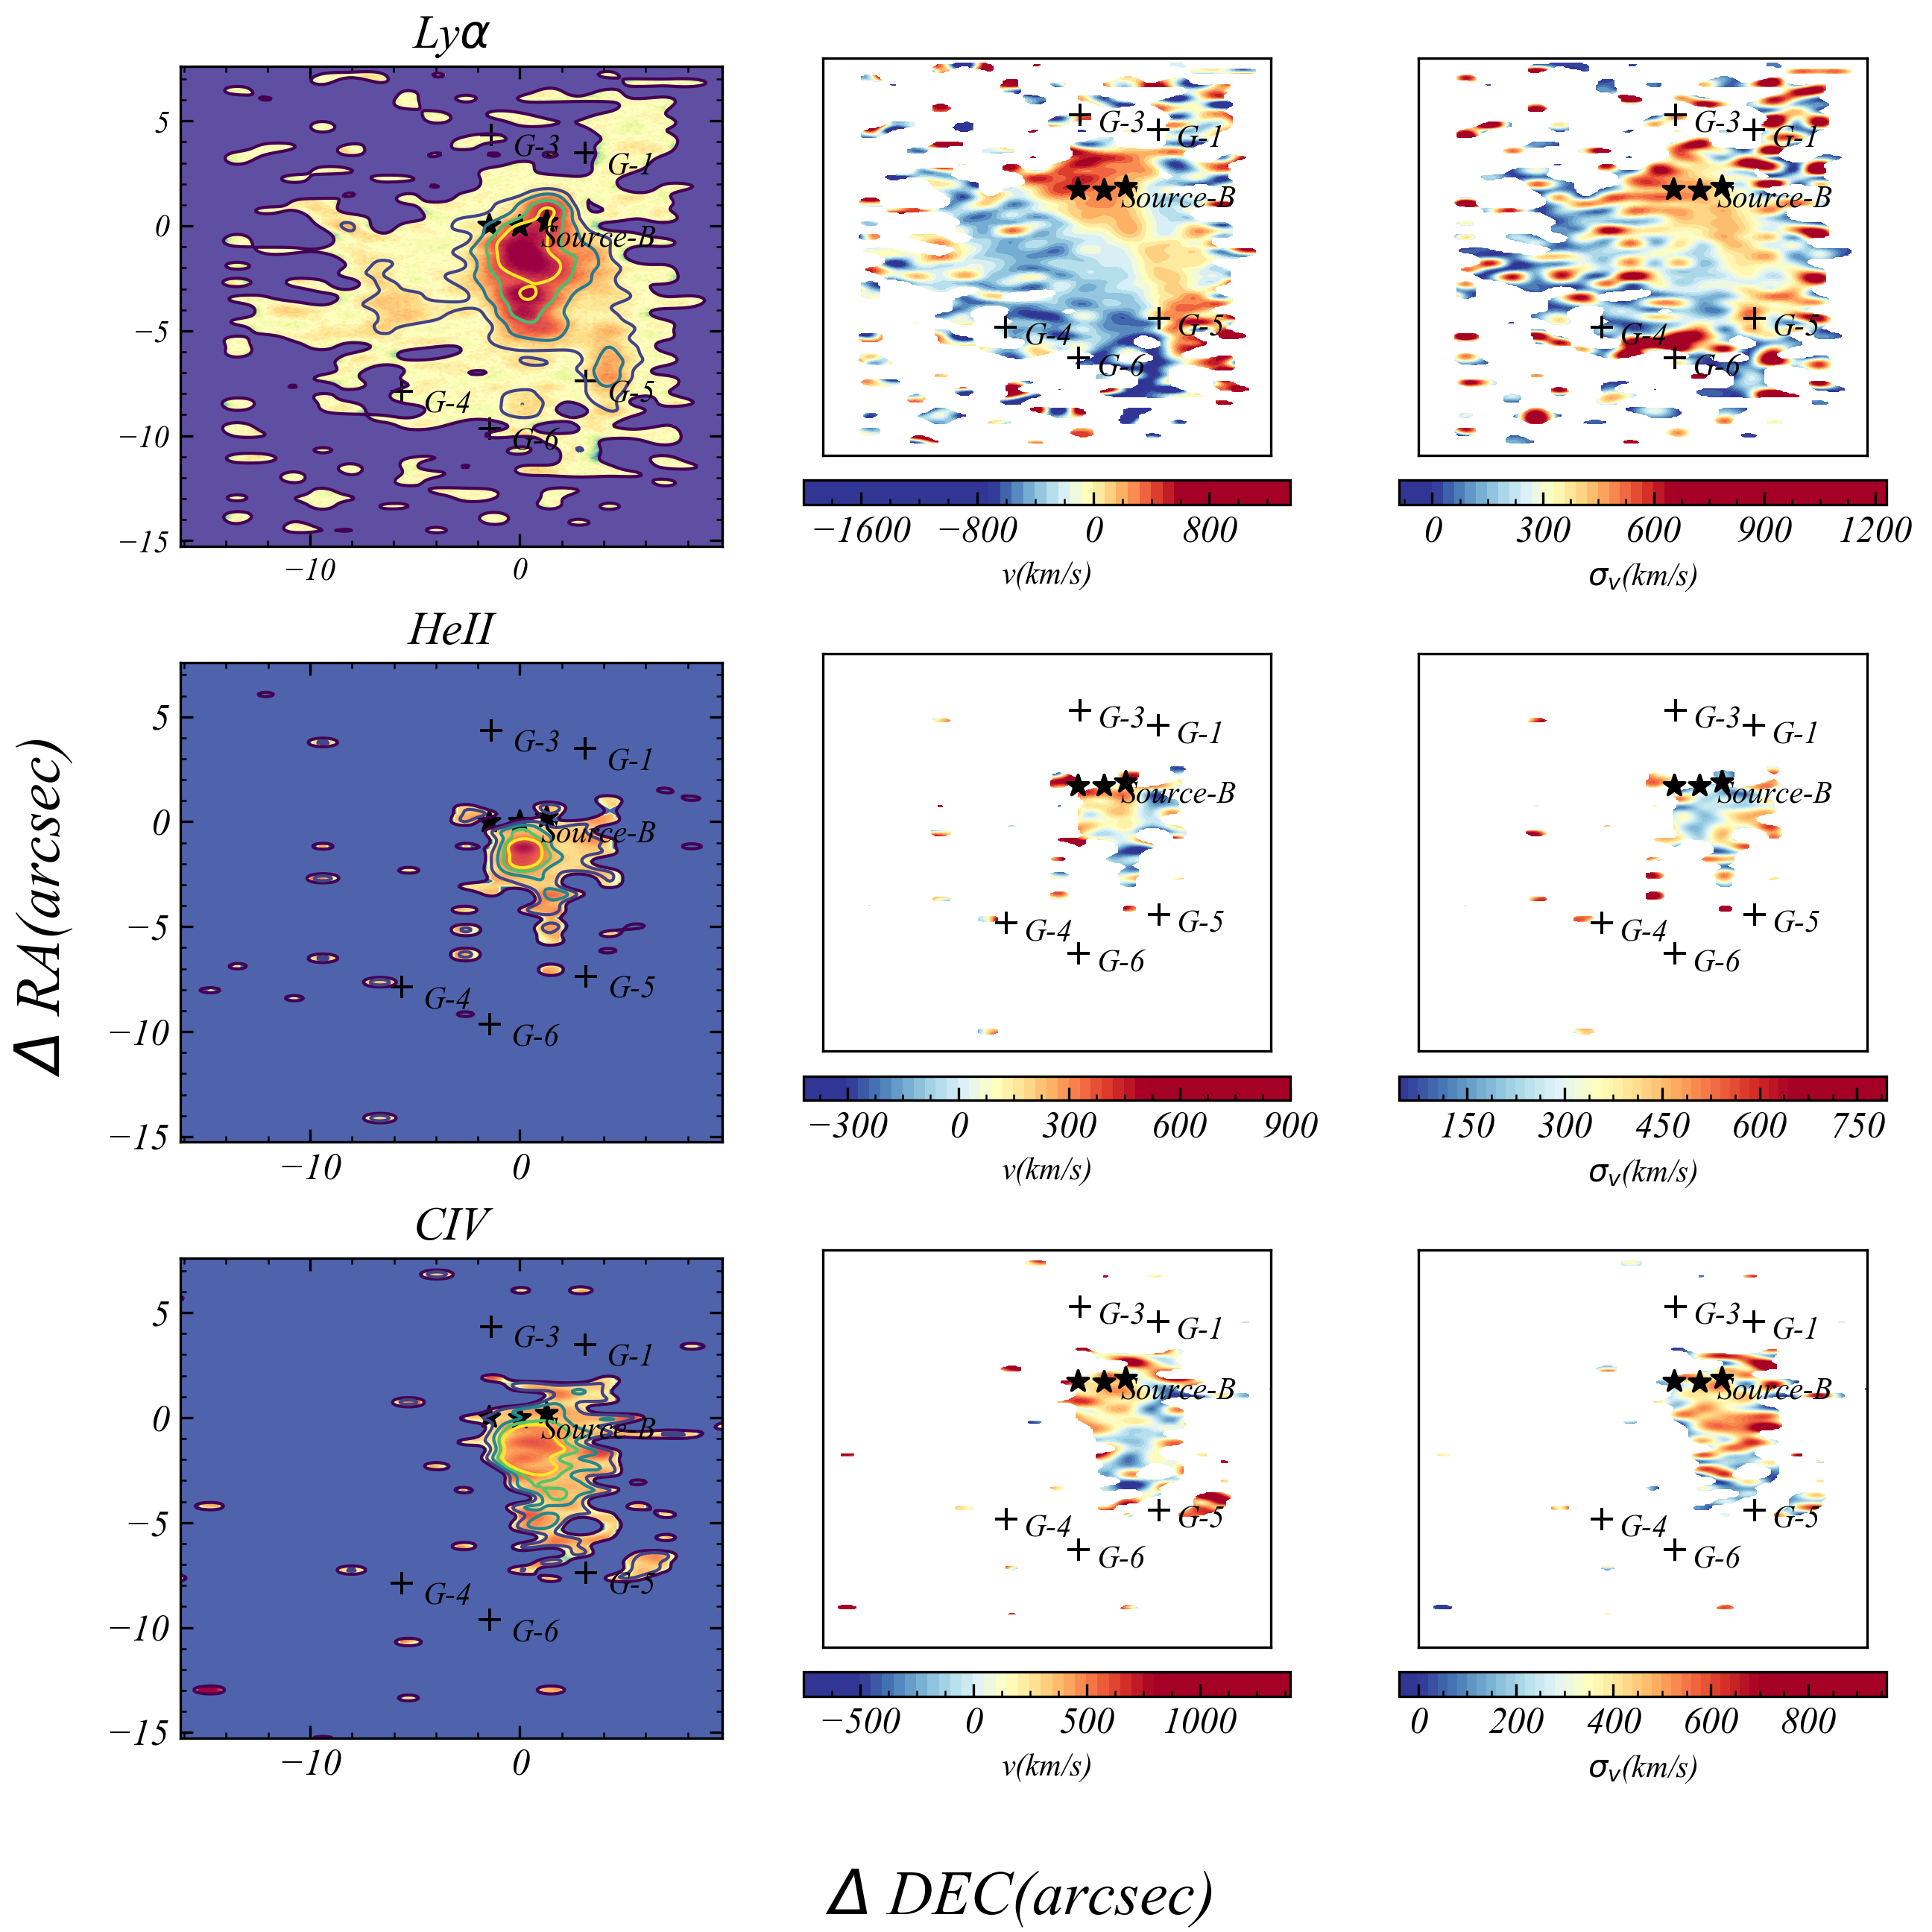
\includegraphics[width=\textwidth]{figs/emissionmap}
		\label{kinematicsmap}
		\caption{Left: continuum-subtracted psudo-narrow band images for the 3 emissions. We select regions $> 1.5\sigma$ in each slice and stack these slices together. The contour represent signal-to-noise ratio(SNR), for ly$\alpha$ is ($5\sigma,9\sigma,18\sigma,30\sigma,42\sigma,51\sigma$), for HeII is ($3\sigma,5,9\sigma$) and for CIV is ($4\sigma,7\sigma,9\sigma$). Middle: flux-weighted velocity map with respect to the systemic redshift of MAMMOTH-1. Right: flux-weighted velocity dispersion also with respect to systemic redshift of MAMMOTH-1. We also mark sources in the field with cross.}
	\end{figure*}
	
	Fig. \ref{kinematicsmap} shows the results. Left panel is the continuum-subtracted, pseudo-narrowband image, contour reperesents the SNR levels. Middle panel shows velocity maps and right panel is velocity dispersion map. Ly$\alpha$ shows 2 peaks, one is around source-B the other is around G-5, moreover we we also see significant velocity gradient close to these 2 peaks in ly$\alpha$ velocity map. Besides, dispersion map also reveals relatively large $\sigma_{v}$ around these 2 sources. The 2 clues indicate source-B and G-5 both have outflows. To have a deep insight, we bin the data cube with interval length of 200km/s and show the results in Fig. \ref{slices}. It shows significant separate red and blue component on either side of source-B. As for G-5, the red component is significant but the blue component is relatively weak. 
	\begin{figure*}[htp]
		\centering
		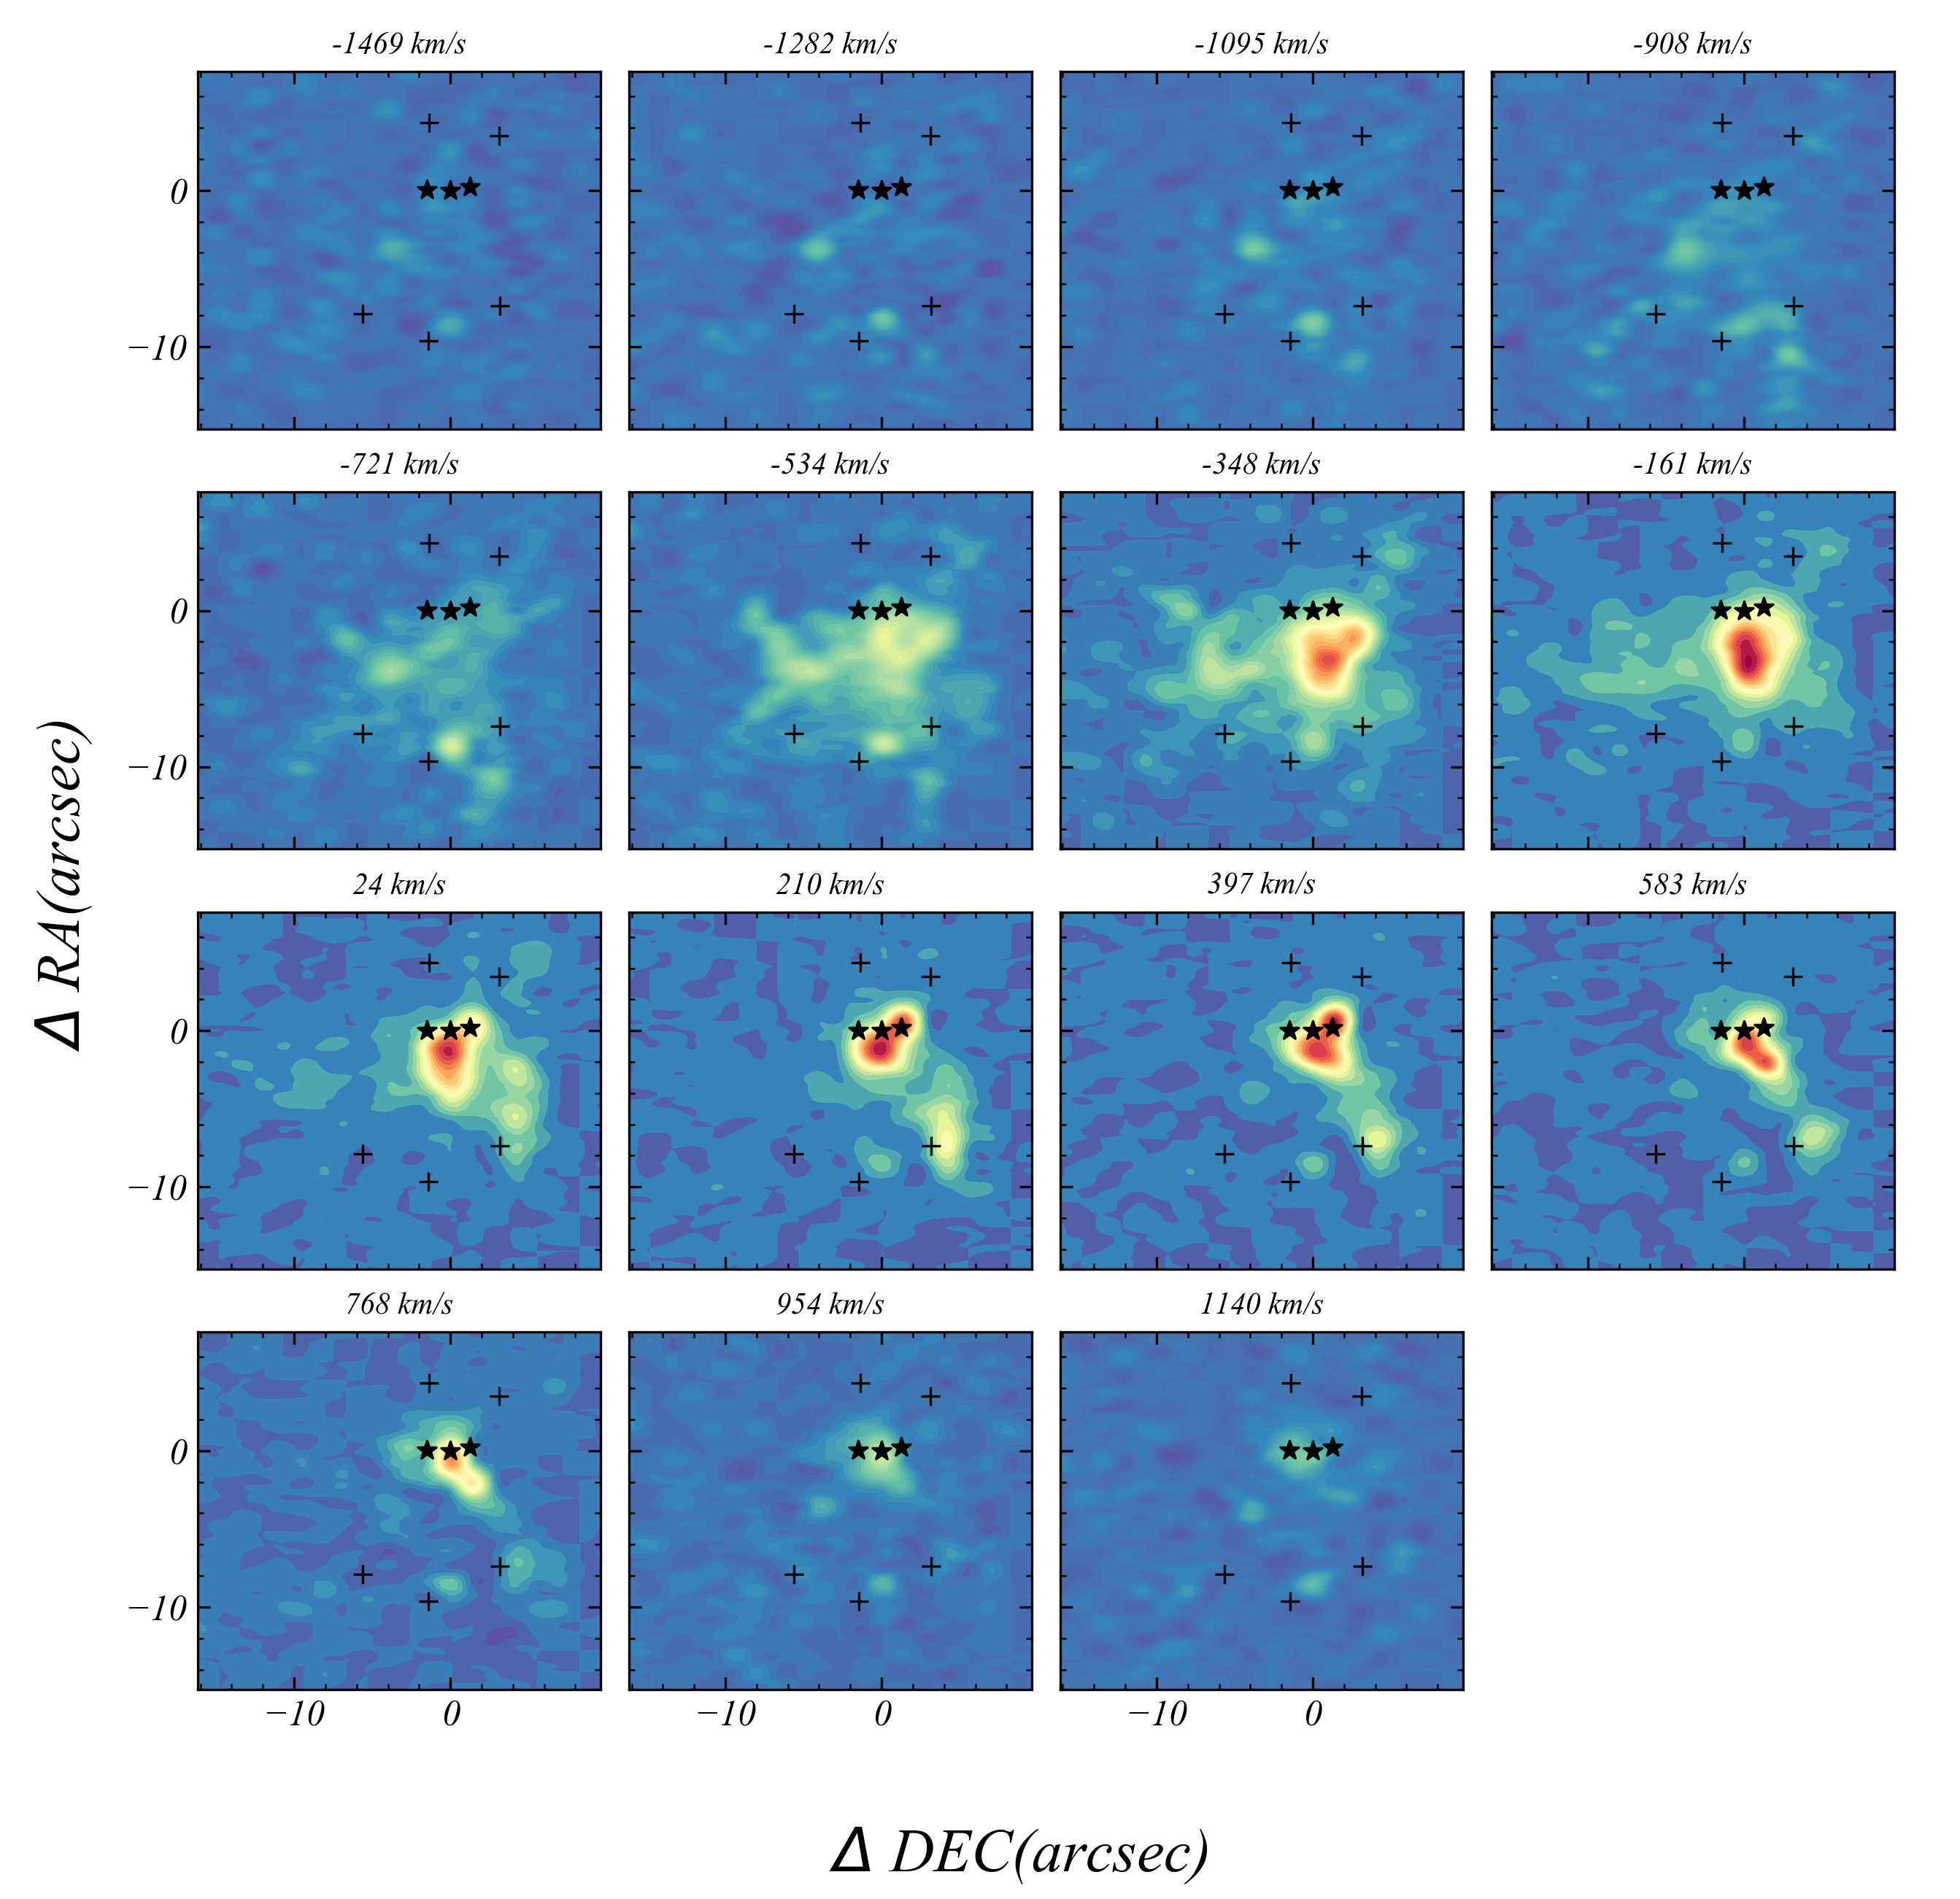
\includegraphics[width=\textwidth]{figs/slices}
		\label{slices}
		\caption{Kinematics of cool gas. It shows signal of ly$\alpha$ emission at different veliocities. We select $\Delta v=187$km/s which corresponds 4$A$  as the bin size of these slices. We extract these slices within the range $4000A-4040A$, for each image here, we use the mean velocity of the bin as title for each image. It shows significant red and blue component on either side of source-B.}
	\end{figure*}
	
	To further explore the physical mechanism here, we extract spectra from different regions of ly$\alpha$ nebula and construct a "spectral map", Fig.\ref{specmap} shows the result. We construct aperture with radius of 1$arcsec^{2}$ and extract spectra from different part of Ly$\alpha$ neubulae. We also fit lines with one-component gaussian function and show the fitting parameter in Tab. \ref{fitpara}. We clearly see in some regions close to source-B the dispersion is really large even $>600$km/s which corresponds to FWHM$>1400$km/s. It's hard to imagine anything other than an outflow could cause such a large dispersion.
%	We number 2''$\times$2'' windows from 0 to 19 and extract spectra, these emission lines are fitted with multi-component gaussian function. \ref{fig:specmap} mainly provide us with five pieces of information. (i) we do see multi-component ly$\alpha$ emission line in some areas(window 8,12). (ii) In some area(window 10,11) there's only one component but the velocity dispersion $\approx 500 km/s$ which corresponds to FWHM ~ 1200 km/s. 
	\begin{figure*}[htp]
		\centering
		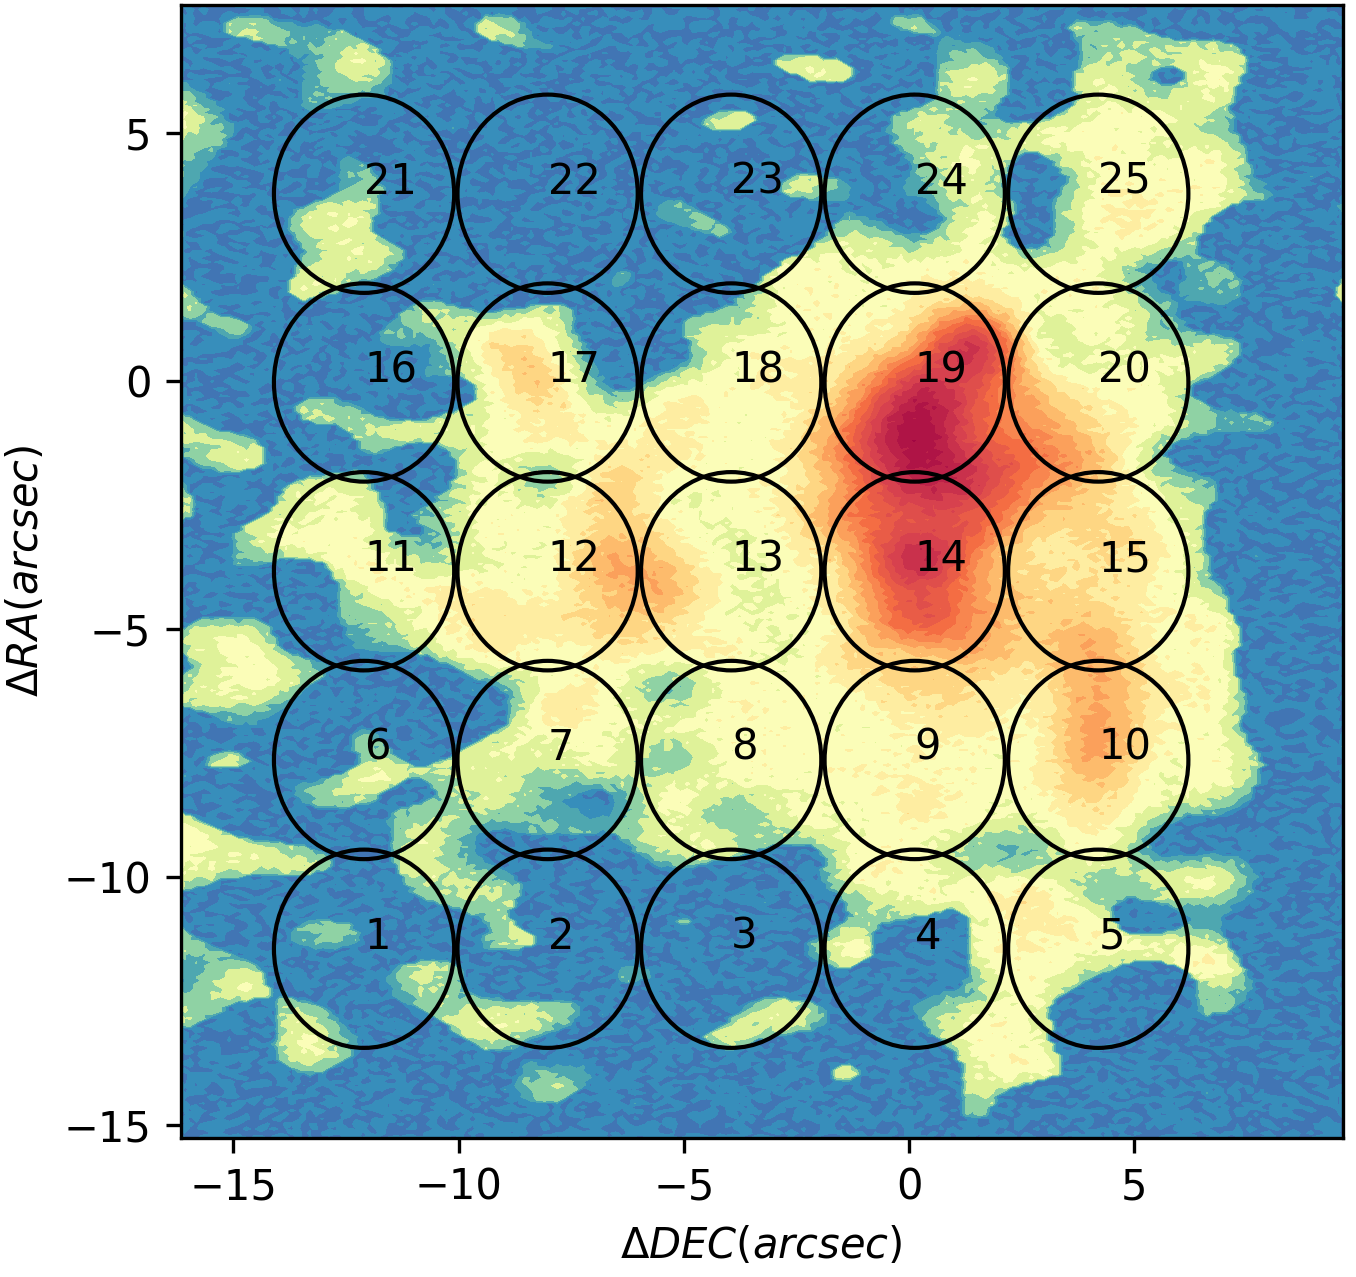
\includegraphics[width=0.5\textwidth]{figs/apertmap.png}
	\end{figure*}
	\begin{figure*}[htp]
		\centering
		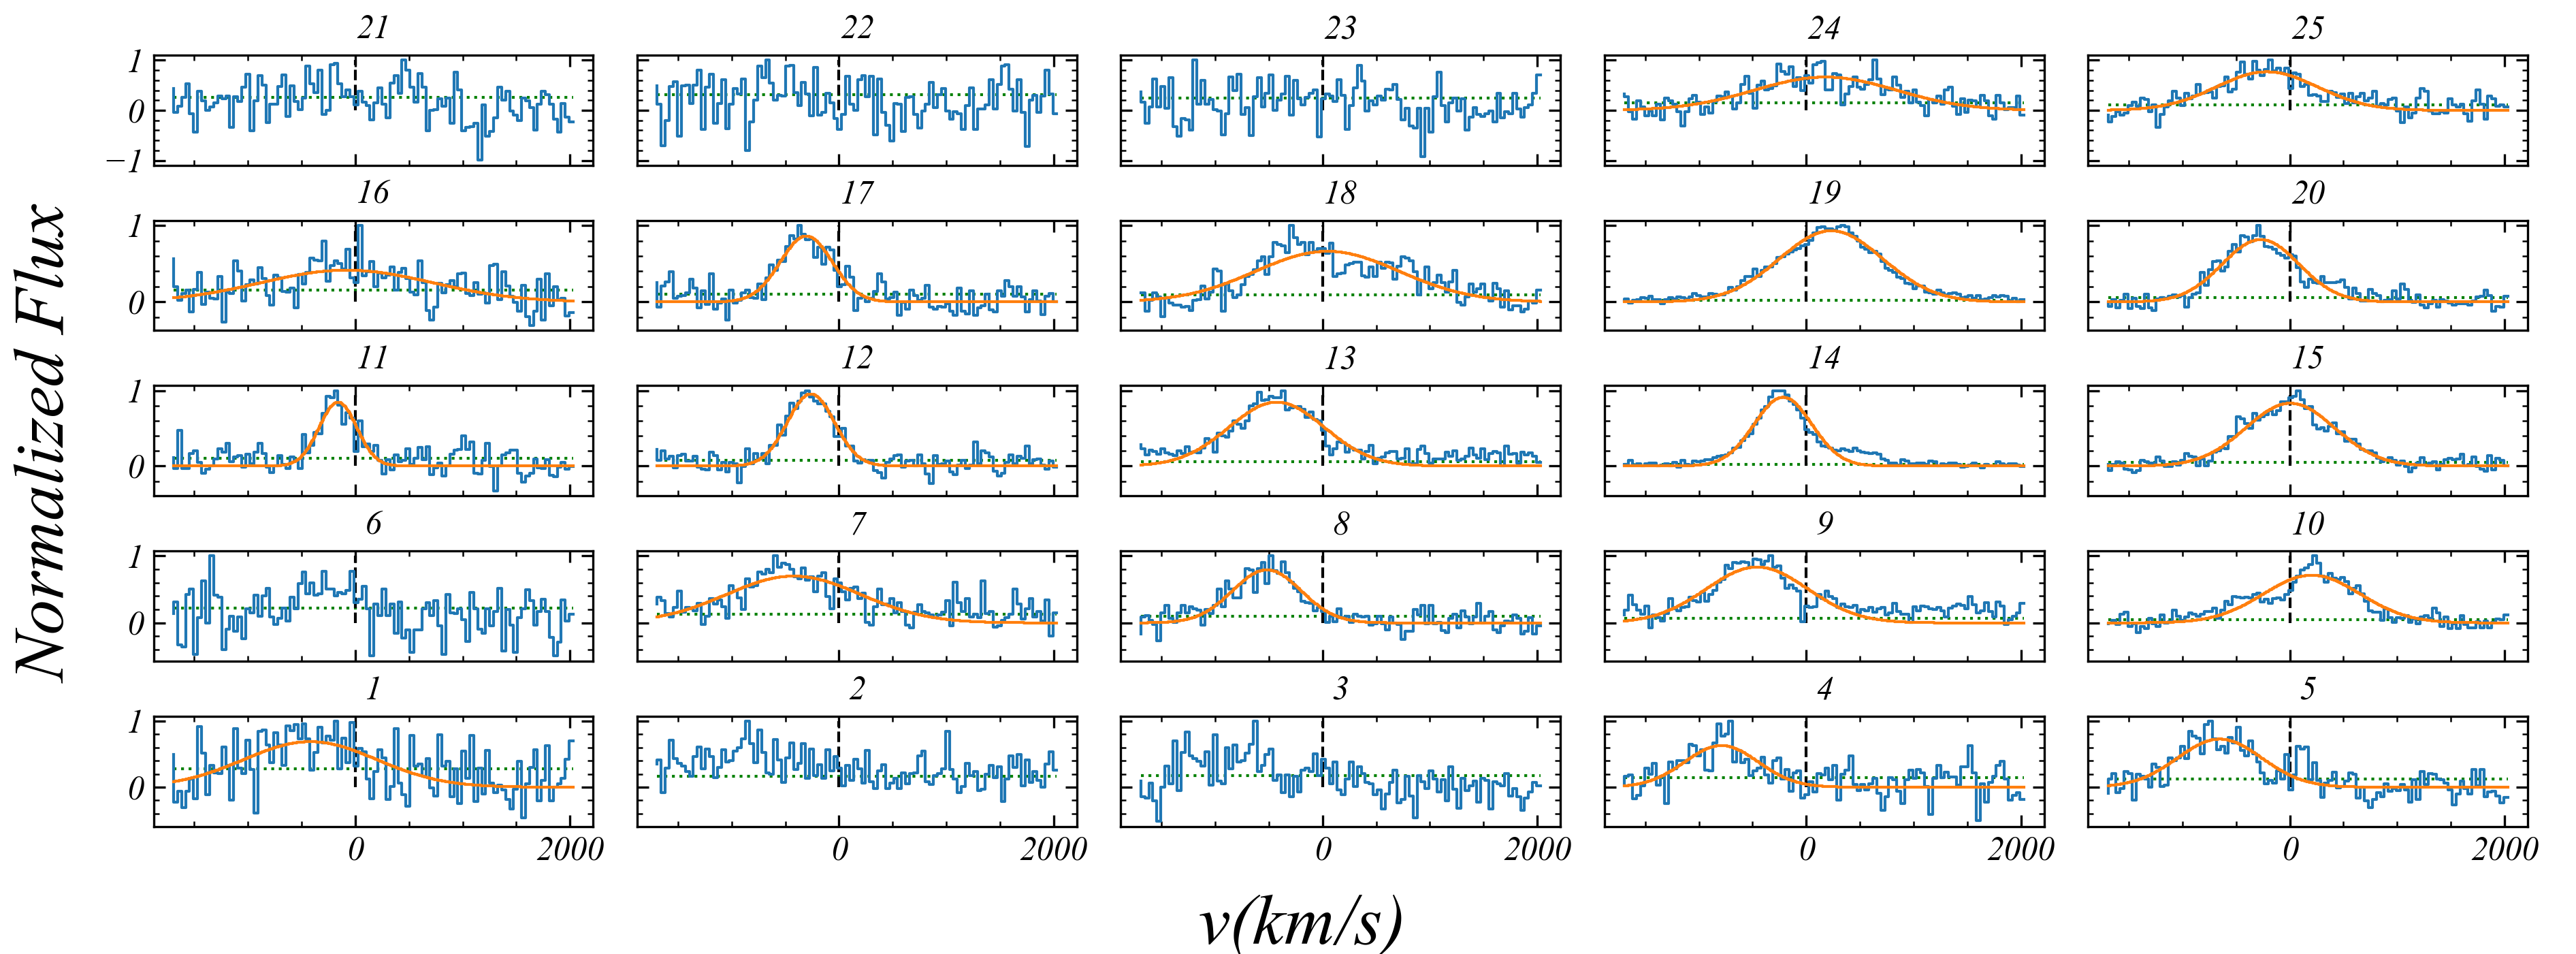
\includegraphics[width=\textwidth,height=0.45\textwidth]{figs/specmap}
		\label{spectralss}
		\caption{Up: Continuum-subtracted psudo narrow band image of ly$\alpha$. We overlay circles on it and number them from 1 to 25.  Low: Continuum-subtracted spectra extracted from individual spatial regions indicated in upper panel. The apertures are circle with radius of 2$arcsec^{2}$. We number the spectra from 1 to 25 which corresponds to circles in upper panel. We fit the emission line with single gaussian function and show it with orange lines. The green lines show the noise level calculated from the high-frequency component of spectra. }
	\end{figure*}
\begin{center}
\begin{table*}[htp]
\begin{tabular}{llllllllllllllllllll}
\hline
\hline
Number & 1    & 4    & 5    & 7    & 8    & 9    & 10   & 11   & 12   & 13   & 14   & 15  & 16   & 17   & 18   & 19   & 20   & 24   & 25   \\
\hline
Velocity(km/s)   & -416 & -785 & -649 & -419 & -515 & -453 & 208  & -157 & -257 & -424 & -211 & 9    & -75  & -300 & 49   & 236  & -267 & 182  & -208 \\
Dispersion(km/s) & 618  & 342  & 392  & 626  & 319  & 474  & 450  & 174  & 219  & 444  & 269  & 415  & 799  & 242  & 668  & 481  & 358  & 660  & 472  \\
$f_{norm}$       & 0.69 & 0.63 & 0.73 & 0.70 & 0.79 & 0.83 & 0.71 & 0.84 & 0.95 & 0.85 & 0.91 & 0.83 & 0.41 & 0.86 & 0.66 & 0.93 & 0.81 & 0.66 & 0.77 \\
\hline
\end{tabular}
\label{fitpara}
\end{table*}
\end{center}
	
\end{document}